\subsection{Background: Acoustic Feedback}

Acoustic howling is a phenomenon that arises due to an acoustic feedback path, specifically, the occurrence of acoustic coupling between a loudspeaker and a microphone. This coupling results in the microphone picking up the sound signal emitted by the loudspeaker, and subsequently, this captured signal is fed back to the loudspeaker after undergoing amplification. This particular occurrence is commonly referred to as acoustic feedback.

From the perspective of a closed-loop system, the occurrence of howling is contingent upon meeting certain conditions of instability. The analysis of these conditions is rooted in the Nyquist stability criterion, which can be derived from an examination of the closed-loop frequency response of the system illustrated in Figure \ref{fig:system_diagram_original}.

\begin{figure}[ht]
    \centering
    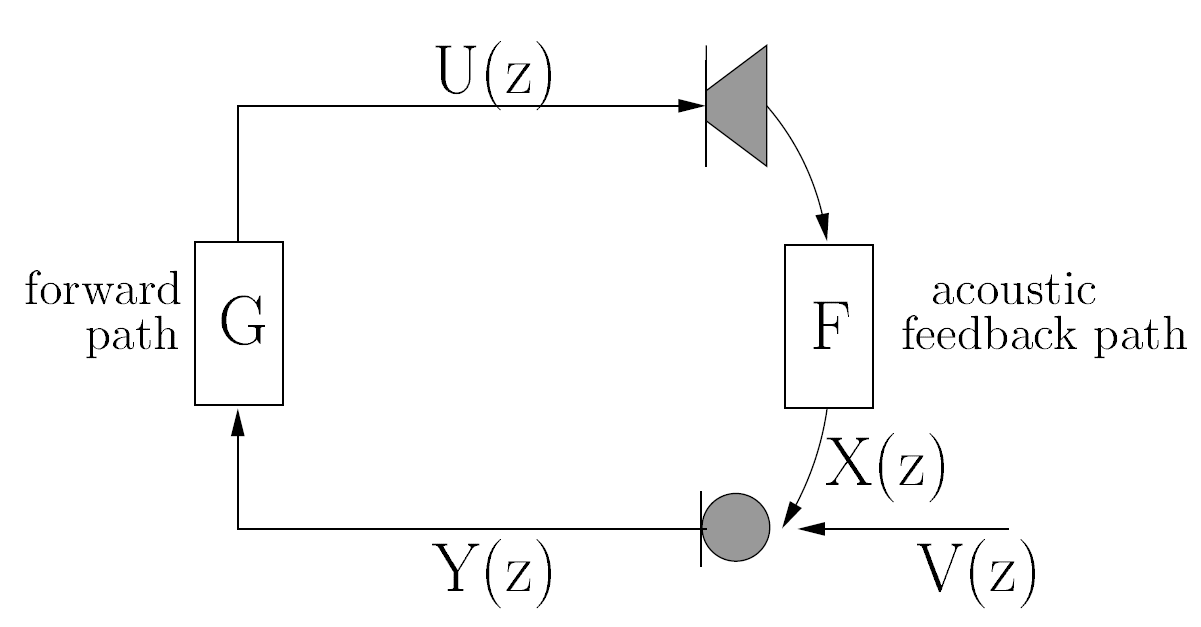
\includegraphics[width=0.8\columnwidth]{images/system_digram_original.png}
    \caption{Acoustic feedback problem in a 1-microphone/1-loudspeaker setup\cite{7077829}}
    \label{fig:system_diagram_original}
\end{figure}

\subsection{Problem statement}
\subsubsection{Assumptions}

For our analysis, we focus on a single-channel setup, consisting of one loudspeaker and one microphone, with the following characteristics:

\begin{itemize}
    \item Linear and flat response in the loudspeaker.
    \item Linear and flat response in the microphone.
    \item Linear and flat response in the forward path (amplifier).
    \item Linear but non-flat response in the acoustic feedback path.
\end{itemize}

The desired system transfer function is:
\begin{equation}
    \frac{U(z)}{V(z)} = G(z)
\end{equation}

The resulting closed-loop system transfer function is:
\begin{equation}
    \frac{U(z)}{V(z)} = \frac{G(z)}{1 - G(z) F(z)}
\end{equation}

This system configuration is prone to spectral coloration, acoustic echoes, and, notably, the risk of instability—our primary concern. The loop response is quantifiable by the loop gain $\mid G(e^{i \omega}) F(e^{i \omega})\mid$ and loop phase $\angle G(e^{i \omega}) F(e^{i \omega})$.

\subsubsection{Nyquist Stability Criterion}:
If a radial frequency $\omega$ exists where

\begin{equation}
    \left\{\begin{array}{l}
    \left|G\left(e^{i \omega}\right) F\left(e^{i \omega}\right)\right| \geq 1 \\
    \angle G\left(e^{i \omega}\right) F\left(e^{i \omega}\right)=n 2 \pi, n \in \mathbb{Z}
    \end{array}\right.
\end{equation}

then the closed-loop system is unstable. Excitation of the unstable system at this critical frequency $\omega$ will result in oscillation at the frequency, known as howling.

An example of closed-loop system instability is depicted in Figure \ref{fig:input_spectrogram}.

\subsubsection{Target}

\begin{figure}[ht]
    \centering
    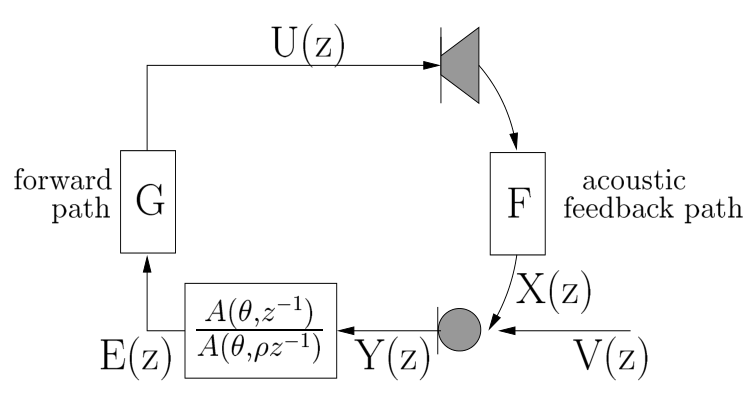
\includegraphics[width=0.8\columnwidth]{images/system_digram_anf.png}
    \caption{Including an adaptive notch filter in the 1-microphone/1-loudspeaker
setup\cite{7077829}}
    \label{fig:system_diagram_anf}
\end{figure}

The primary goal of this project is to remove feedback oscillations in closed-loop systems as shown in Figure \ref{fig:system_diagram_anf}. Our approach involves initially addressing a single narrow-band noise source in a signal using a simplified method with a fixed pole radius, denoted as $\rho$. We then advance this technique by adopting an iteratively adaptive $\rho$, enhancing the filter's effectiveness. 

In our implementation of these filters, we have utilized both C and assembly languages on a C5515 development board. To assess performance in an offline setting, we tested the filters with a specifically generated signal, analyzing the time-spectrum of both the input and the output to evaluate the efficacy of the noise reduction. Additionally, we conducted real-time system testing, where a microphone served as the input and a speaker was used as the output. This setup allowed us to observe the filter's performance in a live audio processing environment, demonstrating its capability to effectively manage feedback oscillations.


\subsection{Adaptive Notch Filtering}
The objective of acoustic feedback control in audio systems is to either completely eliminate acoustic coupling or to partially reduce howling in loudspeaker signals. This can be achieved through manual control techniques such as optimal microphone and loudspeaker placement, pre-emptive room equalization with 1/3 octave graphic EQ filters, and targeted suppression of specific room modes using notch filters. Alternatively, automatic control requires no sound engineer intervention and encompasses various methods: gain reduction for adjusting gain post-howling detection, phase modulation methods for loop gain smoothing, spatial filtering through adaptive microphone beamforming to lessen direct coupling, and room modeling involving adaptive inverse filtering and feedback cancellation. Within these, the gain reduction approach, further classified into automatic gain control, automatic equalization, and notch filtering, is particularly noteworthy for its application in full-band gain reduction and specific frequency band suppression. In this project, we chose gain reduction method by utilizing the adaptive notch filter.

Firstly, let us recall the biquad filter in the $z$-domain without any constraints:
\begin{equation}
    H\left(z^{-1}\right)=\frac{b_o+b_1 z^{-1}+b_2 z^{-2}}{1+a_1 z^{-1}+a_2 z^{-2}}
\end{equation}
which for $b_o=1$, can be expressed in polar coordinates (in the complex plane) in terms of a zero radius, $\zeta$, and zero angle $\omega_z$, and a pole radius, $\rho$, and pole angle, $\omega_p$ as follows
\begin{equation}
    H\left(z^{-1}\right)=\frac{\left(1-\zeta e^{j \omega_z} z^{-1}\right)\left(1-\zeta e^{-j \omega_z} z^{-1}\right)}{\left(1-\rho e^{j \omega_p} z^{-1}\right)\left(1-\rho e^{-j \omega_p} z^{-1}\right)}
\end{equation}

In order to convert this filter into a more suitable form where its coefficients can be adapted, two constraints need to be subsequently introduced.

The first of these constraints is to make the poles and zeros lie on the same radial line, defined by angle $\omega$ in the complex plane (see Fig. 1), i.e. $\omega_z=\omega_p=\omega$. These poles and zeros must also lie completely within the unit circle, where the zeros would be in between the poles and the unit circle in order to define a notch filter. The intuition behind this is that placing a zero near to the unit circle would attenuate all the frequency components in the neighbourhood of the angular frequency, $\omega$, defining that particular radial line. Placing a pole on the same radial line then creates a resonance at $\omega$, with the bandwidth of the notch filter becoming narrower as $\rho \rightarrow \zeta$.

The second constraint on the biquad filter is to let the zeros all lie on the unit circle so that $\zeta=1$. In this case the frequency component at $\omega$ would be completely attenuated and the pole at the same radial line would once again create a resonance at $\omega$, with the bandwidth of the notch filter becoming narrower as $\rho \rightarrow 1$.

Imposing these constraints on the biquad filter of (3), results in the constrained biquad filter:
\begin{equation}
    \begin{aligned}
     H\left(z^{-1}\right) & =\frac{\left(1-e^{j \omega} z^{-1}\right)\left(1-e^{-j \omega} z^{-1}\right)}{\left(1-\rho e^{j \omega} z^{-1}\right)\left(1-\rho e^{-j \omega} z^{-1}\right)} \\
    & =\frac{1-2 \cos (\omega) z^{-1}+z^{-2}}{1-2 \rho \cos (\omega) z^{-1}+\rho^2 z^{-2}} \\
    & =\frac{1-a z^{-1}+z^{-2}}{1-\rho a z^{-1}+\rho^2 z^{-2}}
    \end{aligned}
\end{equation}
where $a \triangleq 2 \cos (\omega)=2 \cos \left(2 \pi f / f_s\right)$ is the only parameter we need to estimate (since it appears in both the numerator and denominator) and is directly related to the centre frequency, $f$, of the notch filter. Consequently, by adapting the $a$ coefficient, the centre frequency of the notch filter also changes resulting in an ANF.\cite{ali2023frequency}

\subsection{ANF-LMS Algorithm}

The second-order constrained Adaptive Notch Filter (ANF) utilizing a Direct-Form II architecture is optimized for memory efficiency, a critical aspect in digital signal processing. This architecture segregates the filter into a feedforward Finite Impulse Response (FIR) section and a feedback Infinite Impulse Response (IIR) section. Specifically designed to target and diminish certain frequencies, such as those contributing to acoustic feedback, the filter adapts its coefficients in response to signal variations. The adaptation is achieved by updating the FIR coefficients according to the input signal and a chosen algorithm like LMS, then reflecting these changes in the IIR section. This mirroring ensures that the filter consistently suppresses the intended frequencies and remains stable, even when the characteristics of the noise or feedback evolve over time. This method not only streamlines the adaptation process but also enhances the filter's stability in dynamic acoustic environments.

The Least Mean Squares (LMS) algorithm is used for the coefficient update\cite{vanwaterschoot2014}, ensuring efficient and effective adaptation to the changing acoustic environment. It adapts over time by adjusting its parameters to minimize the difference between the filtered and actual signals. The algorithm inputs include the step size $μ$, which affects convergence speed; initial and final pole radii $\rho(0)$ and $\rho(\infty)$, which determine the notch filter's initial width and its convergence target; the decay time constant $\lambda$, guiding the rate at which $\rho(t)$ approaches $\rho(\infty)$; and the input signal $y(t)$. The output $x(t)$ is the filtered signal, and $a(t)$ represents the adaptive filter coefficients. At each iteration $t$, the algorithm updates the pole radius $\rho(t)$, computes the current filtered output $x(t)$, calculates the error $e(t)$ between the filtered and actual signals, and then adjusts the filter coefficients $a(t)$ to reduce this error, iteratively optimizing the filter's performance to suppress the noise.

\begin{algorithm}
\caption{2$^{\text{nd}}$ order ANF-LMS algorithm}
\begin{algorithmic}[1]
\State \textbf{Input:} step size $\mu$, initial pole radius $\rho(0)$, final pole radius $\rho(\infty)$, exponential decay time constant $\lambda$, input data $\{y(t)\}_{t=1}^N$, initial conditions $x(0), x(-1), a(0)$
\State \textbf{Output:} 2$^{\text{nd}}$ order ANF parameter $\{a(t)\}_{t=1}^N$
\For{$t = 1, \ldots, N$}
    \State $\rho(t) = \lambda \rho(t - 1) + (1 - \lambda) \rho(\infty)$
    \State $x(t) = y(t) + \rho(t) a(t - 1) x(t - 1) - \rho^2(t) x(t - 2)$
    \State $e(t) = x(t) - a(t - 1) x(t - 1) + x(t - 2)$
    \State $a(t) = a(t - 1) + 2 \mu e(t) x(t - 1)$
\EndFor
\end{algorithmic}
\end{algorithm}


